% ScoutRoute paper draft. Built on the official VLDB 2027 / PVLDB Vol. 20
% template. The bundled acmart.cls and pvldb.sty must not be modified.
\documentclass[sigconf, nonacm]{acmart}

%%% do not modify the following VLDB block %%
%%% VLDB block start %%%
\usepackage{pvldb}
%%% VLDB block end %%%

\usepackage{amsmath}
\usepackage{booktabs}
\usepackage{multirow}
\usepackage{xcolor}
\usepackage{enumitem}
\usepackage{microtype}
\usepackage{xspace}
\usepackage{tikz}
\usetikzlibrary{arrows.meta,positioning}

\definecolor{RRBlue}{HTML}{1D4ED8}
\definecolor{RROrange}{HTML}{C2410C}
\definecolor{RRGreen}{HTML}{047857}
\definecolor{RRGray}{HTML}{4B5563}

\renewcommand\vldbdoi{XX.XX/XXX.XX}
\renewcommand\vldbpages{XXX-XXX}
% TODO(submission): an EA&B submission must provide the artifact URL initially.
\renewcommand\vldbavailabilityurl{}

\newcommand{\system}{\textsc{ScoutRoute}\xspace}
\newcommand{\nano}{\textsc{Nano}\xspace}
\newcommand{\mini}{\textsc{Mini}\xspace}
\newcommand{\bc}{\textsc{BC}\xspace}
\newcommand{\mo}{\textsc{MO}\xspace}
\newcommand{\no}{\textsc{NO}\xspace}
\newcommand{\bw}{\textsc{BW}\xspace}
\newcommand{\todo}[1]{\textcolor{red!70!black}{\textbf{TODO:} #1}}

\begin{document}

\title{ScoutRoute: Active Data Acquisition and Cost-Derived Scoring for Lightweight Soft-Prompt Routing [Experiment, Analysis \& Benchmark]}

% PVLDB is single blind. Replace all fields below before submission.
\author{Author Name(s) --- TODO}
\affiliation{%
  \institution{Institution --- TODO}
  \city{City --- TODO}
  \country{Country --- TODO}
}
\email{author@example.edu}

\begin{abstract}
Semantic query engines increasingly execute natural-language operators over
large collections, making language-model choice a database execution decision.
A small model is inexpensive but occasionally fails on precisely the tuples for
which a stronger model is correct. These critical cases are rare, so aggregate
validation accuracy can favor a cheap router that silently loses recoverable
answer quality. We present \system, an outcome-aware routing framework built
around two mechanisms. First, disagreement-guided acquisition executes both
candidate models on an unlabeled pool, prioritizes examples on which their
answers differ while retaining a coverage sample of agreements, and requests
human gold labels only for the selected subset. This observable policy enriches
the rare one-model-only cases that determine routing quality while reducing
gold-annotation demand. Second, a cost-derived score assigns
a correct route inverse expected execution cost and an incorrect route zero,
providing an auditable value for every routing decision.

The primary router is a continuous soft prompt over a frozen compact encoder
trained only with inverse-expected-cost weighted cross-entropy. Disagreement
selection supplies the rare recoverable failures; no outcome-specific weight is
hand tuned. Only
the prompt embeddings and a two-class head are updated---3,074--13,826
parameters in our configurations---and online routing requires neither
autoregressive generation nor a multi-billion-parameter router. We separately
evaluate reflective discrete instruction optimization as an independent
alternative that uses the same cost score for feedback. Across SemBench Movie
and MMLU-Pro Computer Science, our acquisition studies show stronger coverage
of decision-critical outcomes under a fixed human-label budget. In a 200-item
Computer Science pool, labeling 100 disagreement-prioritized candidates covers
all 19 Mini-only cases, whereas random selection covers 53.1\% on average.
The results motivate data-efficient weighted training and auditable evaluation
of lightweight routers.
\end{abstract}
\maketitle

%%% do not modify the following VLDB block %%
%%% VLDB block start %%%
\vldbtopmatter
%%% VLDB block end %%%

\section{Introduction}

Large language models (LLMs) are becoming physical operators in data systems.
Systems such as LOTUS~\cite{patel2025lotus},
Palimpzest~\cite{liu2025palimpzest}, UQE~\cite{dai2024uqe}, and
DocETL~\cite{shankar2025docetl} expose declarative operators over text, images,
and documents, then choose an execution strategy that trades financial cost,
latency, and result quality.
For a bulk semantic filter or map, even a modest per-tuple price difference is
multiplied by the cardinality of the input relation. Always using the strongest
available model preserves quality but can dominate query cost; always using a
cheap model is efficient but can corrupt downstream filters, joins, and
aggregates.

Model routing treats the model choice as an execution-plan decision. Given a
tuple and operator, a router selects either a cheap model or a stronger model.
Prior LLM-routing work learns this decision from confidence, preferences, or
model features and reports favorable aggregate cost--quality curves
\cite{chen2024frugalgpt,ong2025routellm,gupta2024cascades,jitkrittum2026uniroute}.
Bulk semantic processing creates a particularly unforgiving version of the
problem. The router is invoked repeatedly, failures may be correlated within a
group or predicate, and a small number of false negatives can materially alter
an aggregate. Moreover, the useful training signal is severely imbalanced:
the cheap and strong model agree on most tuples, while the operationally
important event---cheap wrong and strong correct---may be rare.

Consider a sentiment operator over movie reviews. For a review saying
``the film is a disaster, except that it falls into the so-bad-it-is-good
category,'' both models may agree, only the strong model may resolve the
contrast, only the cheap model may happen to be right, or both may fail.
Difficulty alone does not determine the desirable route. A difficult tuple on
which both models fail cannot gain answer accuracy from escalation; conversely,
an apparently simple tuple can be a critical cheap-model failure. A router
trained only on easy/hard labels, overall route accuracy, or class balance
therefore optimizes a surrogate that is misaligned with the query result.

This paper focuses on \emph{lightweight soft-prompt routing} as the primary
way to learn this execution decision. A frozen compact encoder maps each tuple
to a routing representation; only a short continuous prompt and classification
head are trained. This avoids fine-tuning the answer models and, unlike an
LLM-based router, avoids autoregressive decoding by a multi-billion-parameter
model on every tuple. We study discrete natural-language prompt optimization
separately as an interpretable alternative, not as a stage of the soft-prompt
router. Existing prompt optimizers show substantial task gains
\cite{pryzant2023protegi,opsahlong2024mipro,agrawal2025gepa}, but their usual
training data and scalar metrics do not target rare recoverable failures or
distinguish a harmless expensive call from a critical under-escalation.

We introduce \system around two methodological innovations. First,
\emph{disagreement-guided critical-case acquisition} starts from an unlabeled
candidate pool and executes both answer models without revealing gold. It
partitions candidates by whether the two predictions agree, prioritizes
disagreements, retains an agreement sample for coverage, and requests human
gold labels only for the selected subset. Every Mini-only and Nano-only case
must appear in the disagreement stratum, so this observable signal concentrates
annotation on routing-critical examples without inspecting hidden correctness.
On Computer Science QA, both disagreement-guided and random acquisition screen
the same 200 pairs and request 100 human labels. Disagreement-guided selection
covers all 19 Mini-only and all 8 Nano-only cases; random selection covers
53.1\% and 54.8\% on average. Thus the saving is 50\% of human labels relative
to labeling the full screened pool, not a saving in paired model calls. Second,
a \emph{cost-derived route score} assigns inverse expected route cost to a
correct route and zero to an incorrect route, making every routed decision
auditable in common units. The primary soft-prompt router is trained only with
inverse-expected-cost weighted cross-entropy. Disagreement enrichment, rather
than a hand-tuned Mini-only weight, ensures that rare recoverable errors
influence training. The cost score reports the resulting cost--quality frontier
and supplies feedback to the separate GEPA adapter; it is not a second
soft-prompt loss.
The empirical finding is deliberately more nuanced than ``routing saves
cost.'' The lightweight soft-prompt router has only 3,074--13,826 trainable
parameters and provides a smooth validation cost--quality curve. On historical
Movie splits, outcome enrichment and cost-weighted CE produce configurations
near all-Mini accuracy while avoiding 15.85--34.15\% of Mini calls. However, the
locked fresh evaluation shows that the apparent frontier does not robustly
reproduce: the mean router loses 1.33 accuracy points and Mini-call savings vary
by 24 points across seeds. More soft-prompt tokens do not monotonically help.
The independent discrete router has a different failure mode: hard routing
collapses to all-Nano, and a calibrated verbal risk score only partly repairs
it. Computer Science confirms that preserving all-Mini accuracy remains
expensive under the present data budget.

Our methodological novelty is concentrated in the first two contributions:

\begin{itemize}[leftmargin=*]
  \item \textbf{Disagreement-guided acquisition of critical routing data.}
  We screen an unlabeled pool with both answer models, prioritize candidates
  whose answers disagree, retain agreement coverage, and obtain human gold
  labels only for the selected subset. The observable split enriches the
  one-model-only cases that control router accuracy and reduces annotation
  demand without using correctness during selection.
  \item \textbf{Weighted soft-prompt routing with cost-derived evaluation.}
  Paired execution assigns both routes an auditable score from correctness and
  expected route cost. Inverse-expected-cost weighted cross-entropy trains only
  3,074--13,826 parameters over a frozen compact encoder. The score also
  supplies feedback through a separate GEPA adapter.

  \item \textbf{Independent comparison and careful evaluation.} Across 1,012 paired Movie reviews, a locked 200-row fresh set,
  and 410 Computer Science questions, we compare the lightweight soft-prompt
  method against reflective discrete instructions, loss designs, acquisition
  policies, and validation thresholds.
\end{itemize}

The current draft is an Experiment, Analysis \& Benchmark submission because
its strongest result is the controlled characterization of reliability, not a
claim that one prototype dominates all baselines. The final artifact will
release split manifests, paired outcomes, optimization traces, and scripts
needed to reproduce every table.

\section{Prompt Optimization Overview}
\label{sec:overview}

\begin{figure*}[t]
  \centering
  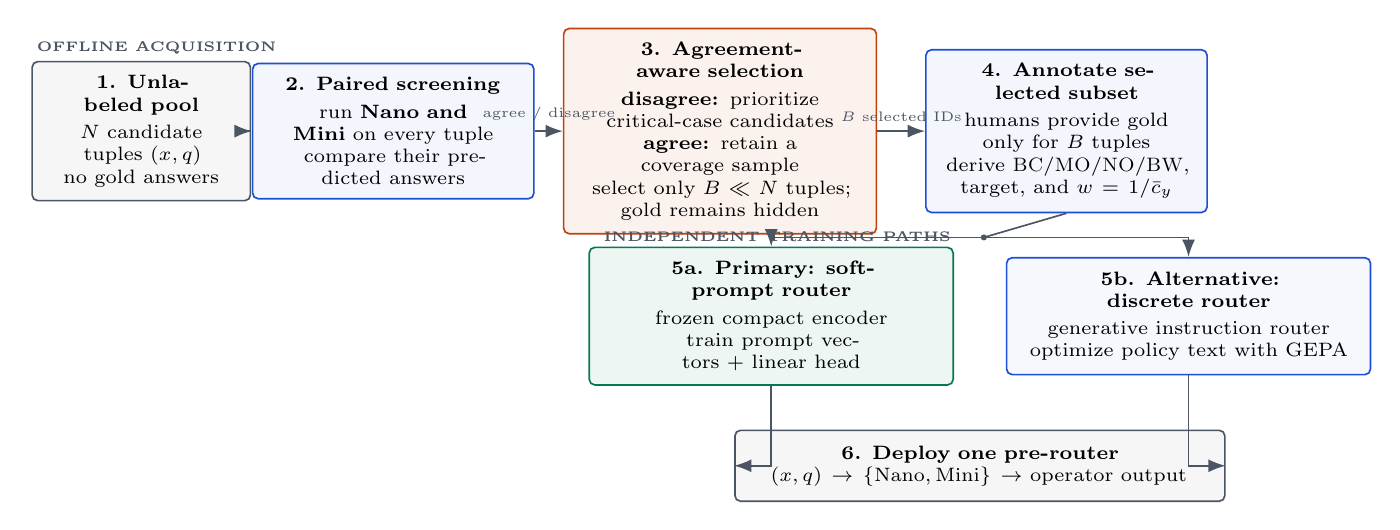
\begin{tikzpicture}[
    font=\scriptsize,
    >={Latex[length=2.2mm]},
    flow/.style={->, semithick, draw=RRGray},
    box/.style={draw=RRGray, rounded corners=2pt, semithick, align=center,
      inner xsep=6pt, inner ysep=5pt},
    pool/.style={box, fill=RRGray!5, text width=2.35cm, minimum height=1.45cm},
    screen/.style={box, draw=RRBlue, fill=RRBlue!5,
      text width=3.15cm, minimum height=1.45cm},
    acquire/.style={box, draw=RROrange, fill=RROrange!7,
      text width=3.55cm, minimum height=1.55cm},
    data/.style={box, draw=RRBlue, fill=RRBlue!5,
      text width=3.15cm, minimum height=1.55cm},
    soft/.style={box, draw=RRGreen, fill=RRGreen!7,
      text width=4.2cm, minimum height=1.35cm},
    discrete/.style={box, draw=RRBlue, fill=RRBlue!4,
      text width=4.2cm, minimum height=1.35cm},
    deploy/.style={box, fill=RRGray!5, text width=5.8cm, minimum height=0.9cm}
  ]
    \node[pool] (pool) at (-0.1,1.7)
      {\textbf{1. Unlabeled pool}\\[2pt]
       $N$ candidate tuples $(x,q)$\\no gold answers};

    \node[screen] (screen) at (3.1,1.7)
      {\textbf{2. Paired screening}\\[2pt]
       run \textbf{Nano and Mini} on every tuple\\
       compare their predicted answers};

    \node[acquire] (acquire) at (7.25,1.7)
      {\textbf{3. Agreement-aware selection}\\[2pt]
       \textbf{disagree:} prioritize critical-case candidates\\
       \textbf{agree:} retain a coverage sample\\
       select only $B\ll N$ tuples; gold remains hidden};

    \node[data] (data) at (11.65,1.7)
      {\textbf{4. Annotate selected subset}\\[2pt]
       humans provide gold only for $B$ tuples\\
       derive \bc/\mo/\no/\bw, target, and $w=1/\bar c_y$};

    \node[soft] (soft) at (7.9,-0.65)
      {\textbf{5a. Primary: soft-prompt router}\\[2pt]
       frozen compact encoder\\train prompt vectors + linear head};

    \node[discrete] (discrete) at (13.2,-0.65)
      {\textbf{5b. Alternative: discrete router}\\[2pt]
       generative instruction router\\optimize policy text with GEPA};

    \node[deploy] (deploy) at (10.55,-2.55)
      {\textbf{6. Deploy one pre-router}\\
       $(x,q) \rightarrow \{\text{Nano},\text{Mini}\} \rightarrow$ operator output};

    \draw[flow] (pool) -- (screen);
    \draw[flow] (screen) -- node[above, text=RRGray, font=\tiny]
      {agree / disagree} (acquire);
    \draw[flow] (acquire) -- node[above, text=RRGray, font=\tiny]
      {$B$ selected IDs} (data);
    \coordinate (split) at (10.6,0.35);
    \draw[semithick, draw=RRGray] (data.south) -- (split);
    \fill[RRGray] (split) circle (1.1pt);
    \draw[flow] (split) -| (soft.north);
    \draw[flow] (split) -| (discrete.north);
    \draw[flow] (soft.south) |- (deploy.west);
    \draw[flow] (discrete.south) |- (deploy.east);

    \node[font=\tiny\bfseries, text=RRGray, anchor=south west]
      at (-1.55,2.55) {OFFLINE ACQUISITION};
    \node[font=\tiny\bfseries, text=RRGray, anchor=south west]
      at (5.65,0.18) {INDEPENDENT TRAINING PATHS};
  \end{tikzpicture}
  \caption{End-to-end workflow for an initially unlabeled candidate pool. Nano
  and Mini first screen every candidate without gold labels. Active selection
  prioritizes their disagreements, where recoverable one-model-only cases can
  occur, while retaining agreement examples for coverage. Humans annotate only
  the selected subset; the resulting gold-labeled paired set trains either the
  primary lightweight soft-prompt router or the independent discrete router.
  The two routers are alternatives, not stages of one model.}
  \Description{An unlabeled candidate pool is screened by Nano and Mini. Their
  predicted answers partition the pool into agreement and disagreement strata.
  Active selection prioritizes disagreements and samples some agreements, after
  which humans provide gold labels only for the selected subset. Gold labels and
  the cached paired predictions determine the four correctness outcomes and the
  cost-weighted route targets. This training set branches to two independent
  paths, a lightweight soft-prompt router and a discrete prompt router. Either
  trained router can choose Nano or Mini at deployment time.}
  \label{fig:overview}
\end{figure*}

Figure~\ref{fig:overview} gives the end-to-end workflow when the candidate pool
has no gold answers. The answer-model pair is fixed: $M_N$ denotes the cheap
Nano model and $M_M$ the stronger Mini model. We first execute both models on
the unlabeled pool and partition candidates using the observable event
$\hat z_N(x,q)=\hat z_M(x,q)$. Disagreements receive higher acquisition priority
because every Mini-only and Nano-only case must lie in this stratum; a sampled
agreement subset preserves coverage of ordinary cases and helps control
over-escalation. Selection never inspects an unselected gold answer. Humans then
annotate only the selected $B\ll N$ tuples, at which point the cached pair of
predictions and gold label reveal the \bc/\mo/\no/\bw outcome, route target, and
inverse-cost weight. The resulting agreement-stratified paired set is shared by
two independent training paths: the primary lightweight soft-prompt router and
the discrete prompt router. This workflow saves $N-B$ human annotations, though
it deliberately pays for paired model screening on the full candidate pool.

\paragraph{Soft-prompt router.}
The main \system router prepends $p$ learned embedding vectors to each tuple
and feeds the sequence to a frozen DistilBERT encoder
\cite{sanh2019distilbert}. Only the $p\times768$ prompt matrix and a two-class
linear head are trainable: 3,074, 4,610, 7,682, and 13,826 parameters for
$p\in\{2,4,8,16\}$. The frozen backbone still participates in inference, but
the task-specific state is tiny and routing is a single non-generative encoder
pass rather than autoregressive decoding by a billion-parameter LLM. This makes
the soft-prompt path the practical focus of \system.

Active acquisition determines which tuples train this router. The cost score
defines a hard route target, and its target route receives weight
$1/\bar c_y$. The soft prompt is trained only with the resulting weighted
cross-entropy (Eq.~\ref{eq:weighted-ce}). No outcome-specific constant is
tuned: disagreement enrichment, rather than a manual MO multiplier, ensures that
recoverable failures appear often enough to affect training. A
validation threshold exposes the cost--quality curve without retraining. The
design is inexpensive to retrain and supports multi-seed analysis, though its
learned prompt vectors are not human-readable
\cite{lester2021prompttuning}.
\paragraph{Independent discrete router.}
The discrete method is a separate router, not a component or second stage of
the soft-prompt method. It uses a Qwen3.5-2B generative execution router and a
Qwen3.5-4B reflection model during GEPA optimization. A seed instruction
defines the operator and route tokens; outcome-enriched demonstrations omit
gold labels and answer-model predictions. The adapter attaches route score and
textual feedback to each trace, and GEPA proposes revised policy text
\cite{agrawal2025gepa}. Reflection minibatches contain four examples and the
budget is 20 metric calls.

Hard routing asks for exactly \texttt{nano} or \texttt{mini}; invalid text
falls back to Mini. The scored interface emits raw risk
$\tilde{s}_P(x)\in[0,100]$, which the parser clips and normalizes to
$s_P(x)\in[0,1]$. Validation predicts Mini when $s_P(x)\ge\tau$; reported
thresholds 0.30 and 0.50 therefore use the normalized scale.

\paragraph{Role of the discrete comparison.}
The comparison tests whether the two innovations depend on one router class.
Discrete instructions offer interpretable policies but require substantially
larger generative models and can ignore a verbal rule at generation time. Soft
prompts are compact and directly supervised but can overfit a small validation
set. We report them as two independent methods under shared data and scoring,
never as an ensemble.



% Target length in the official two-column template: approximately 1.5 pages.
\section{Methodology}
\label{sec:method}

\subsection{Routing Objective}

Let $x$ be an input tuple, $q$ a semantic operator, and $M_N,M_M$ the Nano and
Mini answer models. Their predictions are $\hat{z}_N(x,q)$ and
$\hat{z}_M(x,q)$. A pre-router $r_\theta(x,q)\in\{N,M\}$ executes before either
answer model and minimizes expected execution cost subject to a quality target:
\begin{equation}
  \min_\theta\; \mathbb{E}[c_R(x,q)+c_{r_\theta(x,q)}(x,q)]
  \quad\text{s.t.}\quad
  A(r_\theta) \ge A(M_M)-\epsilon,
  \label{eq:constrained}
\end{equation}
where $c_R$ is routing overhead, $A$ is end-to-end answer accuracy, and
$\epsilon$ is an allowed loss. We do not solve Eq.~\ref{eq:constrained}
directly. Training optimizes a scalar surrogate, and a validation-only
candidate/threshold sweep constructs an empirical cost--accuracy frontier. For
an operating point claimed under Eq.~\ref{eq:constrained}, we select the
cheapest validation candidate satisfying the accuracy floor. Historical rows
retain their original calibration rules and are not claimed as direct
solutions of Eq.~\ref{eq:constrained}.

\subsection{Cost-Derived Score Function}

For labeled offline data, paired execution defines outcome
$b(x)=(\mathbb{1}[\hat z_N=z],\mathbb{1}[\hat z_M=z])$, yielding both correct
(\bc), Mini only (\mo), Nano only (\no), or both wrong (\bw). Each cached answer
also records its input and output token counts. Given the price snapshot
$\pi_r^{\mathrm{in}},\pi_r^{\mathrm{out}}$ per million tokens, realized answer
cost is
\begin{equation}
 c_r(x,q)=\frac{\pi_r^{\mathrm{in}}n_{r,x}^{\mathrm{in}}+
                    \pi_r^{\mathrm{out}}n_{r,x}^{\mathrm{out}}}{10^6}.
 \label{eq:realized-cost}
\end{equation}
We estimate each route's expected cost on the training split,
\begin{equation}
 \begin{aligned}
 \bar c_r&=\mathbb{E}_{x\sim\mathcal D_{\mathrm{train}}}[c_r(x,q)]\\
 &=\frac{1}{|\mathcal D_{\mathrm{train}}|}
   \sum_{x\in\mathcal D_{\mathrm{train}}}c_r(x,q)
 \end{aligned}
 \label{eq:expected-cost}
\end{equation}
and use its inverse as the common cost scale:
\begin{equation}
 S_{\mathrm{cost}}(x,r)=
 \frac{\mathbb{1}[\hat z_r(x,q)=z]}{\bar c_r}.
 \label{eq:cost-score}
\end{equation}
A wrong answer receives zero; a correct answer from a lower-expected-cost route
receives a larger score. Multiplying all prices by a common currency conversion
changes score scale but not route ordering.

\begin{table}[t]
  \centering
  \small
  \caption{Cost-derived route score using expected route costs.}
  \label{tab:score}
  \begin{tabular}{lccc}
    \toprule
    Outcome & $S(x,N)$ & $S(x,M)$ & Preferred route\\
    \midrule
    \bc & $1/\bar c_N$ & $1/\bar c_M$ & lower-cost correct model\\
    \mo & $0$ & $1/\bar c_M$ & Mini\\
    \no & $1/\bar c_N$ & $0$ & Nano\\
    \bw & $0$ & $0$ & indifferent; Nano tie-break\\
    \bottomrule
  \end{tabular}
\end{table}
Table~\ref{tab:score} makes the score semantics explicit without a hand-tuned
reward table. A critical under-escalation on \mo forfeits all recoverable
score, while sending \bc to Mini remains correct but earns less whenever
$\bar c_N<\bar c_M$. Neither route can recover \bw; the deployment hard-label rule uses
Nano and reports \bw separately. The \emph{conservative accuracy oracle} in
Tables~\ref{tab:historical-main} and~\ref{tab:fresh} intentionally overrides
this tie and sends \bw to Mini. That convention supplies an accuracy ceiling
with conservative escalation; it is neither the cost-optimal oracle nor the
recommended deployment behavior, and the \bw choice cannot change accuracy.
Invalid discrete output receives zero score and falls back to Mini
operationally. The recorded QA runs use the pricing snapshot embedded in their
artifacts: GPT-4.1 Nano at \$0.10/\$0.40 and Mini at \$0.40/\$1.60 per million
input/output tokens.

\subsection{Disagreement-Guided Critical-Case Acquisition}
\label{sec:active-acquisition}

Let $\mathcal U=\{(x,q)\}_{i=1}^{N}$ be a candidate pool with no revealed gold
answers. We first execute both answer models on every candidate and cache
$\hat z_N(x,q)$ and $\hat z_M(x,q)$. After applying the task's fixed answer
normalizer, these observable predictions define
\begin{equation}
 \begin{aligned}
 \mathcal A &= \{x:\hat z_N(x,q)=\hat z_M(x,q)\},\\
 \mathcal D &= \{x:\hat z_N(x,q)\ne\hat z_M(x,q)\},
 \end{aligned}
 \label{eq:agreement-strata}
\end{equation}
where $\mathcal A$ and $\mathcal D$ are the agreement and disagreement strata.
For exact-label tasks equality is literal; a free-form operator must declare
its equivalence evaluator before acquisition.

Given a human-label budget $B\ll N$, we choose
$\mathcal S_B=\mathcal S_D\cup\mathcal S_A$, with
$\mathcal S_D\subseteq\mathcal D$, $\mathcal S_A\subseteq\mathcal A$, and
$|\mathcal S_D|+|\mathcal S_A|=B$. The policy prioritizes disagreements and
uses a smaller random agreement sample for coverage. Only after
$\mathcal S_B$ is fixed do annotators reveal gold $z$ for those tuples.
Consequently, neither selection nor its tie-breaking can inspect correctness or
the latent \bc/\mo/\no/\bw bucket. Gold and the cached pair then determine the
route target and score in Eq.~\ref{eq:cost-score}.

Disagreement is useful because every \mo and \no case must lie in
$\mathcal D$: one candidate model matches gold and the other does not. These
are the examples that teach when escalation helps and when Nano is preferable.
The disagreement stratum is not itself a correctness label, because \bw can
also disagree. Conversely, agreement examples include ordinary \bc cases that
teach safe Nano routing, as well as shared \bw errors. Retaining agreement
coverage therefore controls over-escalation and exposes systematic shared
failures.

Let $h(x)$ denote the cost of obtaining a human gold answer. Full annotation
and active annotation cost
\begin{align}
 C_{\mathrm{gold}}^{\mathrm{full}} &= \sum_{x\in\mathcal U}h(x),\\
 C_{\mathrm{gold}}^{\mathrm{active}} &= \sum_{x\in\mathcal S_B}h(x).
 \label{eq:annotation-cost}
\end{align}
With constant annotation cost, the gold-label saving is exactly $1-B/N$.
Both active and random selection in our matched comparison pay the same paired
screening cost $\sum_{x\in\mathcal U}(c_N(x)+c_M(x))$. The method therefore
claims human-annotation efficiency, not a reduction in Nano or Mini screening
calls. Its value is that the limited gold budget contains more routing-critical
supervision.

\subsection{Primary Lightweight Soft-Prompt Router}

The primary router uses a frozen encoder rather than a generative LLM. Let
$E(x,q)$ be DistilBERT embeddings and
$V\in\mathbb{R}^{p\times d}$ a trainable soft prompt. The input
$[V;E(x,q)]$ passes through the frozen encoder, and a two-class linear head
produces $p_\theta(r\mid x)$. Only $V$ and the head are updated. For
$d=768$ and $p\in\{2,4,8,16\}$, this is 3,074--13,826 trainable parameters.
The task-specific state is therefore tiny, and the fixed encoder is also
substantially smaller than the separate 2B discrete router. Inference is one
encoder pass with no autoregressive route-token generation.

Active acquisition chooses which paired tuples train the router. The cost score
defines the hard target and the weight for every selected example:
\begin{equation}
 y_i=\arg\max_{r\in\{N,M\}}S_{\mathrm{cost}}(x_i,r),
 \qquad
 w_i=\frac{1}{\bar c_{y_i}},
 \label{eq:cost-target-weight}
\end{equation}
with Nano used when the route scores tie. The soft prompt is trained only with
inverse-expected-cost weighted cross-entropy,
\begin{equation}
 \mathcal{L}_{\mathrm{WCE}}=
 \frac{\sum_i w_i\,
 \ell_{\mathrm{CE}}\!\left(p_\theta(\cdot\mid x_i),y_i\right)}
 {\sum_i w_i}.
 \label{eq:weighted-ce}
\end{equation}
There are no hand-tuned outcome weights and no auxiliary differentiable loss.
Because inverse-cost weighting alone does not upweight rare \mo cases, the
disagreement-guided acquisition stage is responsible for placing enough critical cases
in the training set. This separates two roles cleanly: acquisition controls
rare-case coverage, while Eq.~\ref{eq:weighted-ce} applies one auditable cost
weighting rule to all examples.

Validation enumerates thresholds over $p_\theta(M\mid x)$, selects maximum
answer accuracy with fewer Mini calls as the tie-break, and reports critical
misroutes and realized cost. For Eq.~\ref{eq:constrained}, we instead select the
cheapest validation threshold satisfying the accuracy floor.

\subsection{Independent Reflective Discrete Router}

The discrete method is trained and deployed independently; it is neither an
ensemble member nor a second stage of the soft-prompt router. A candidate $P$
combines an instruction with demonstrations sampled across outcomes. The
2B generative router emits $r_P(x,q)$, while a separate 4B model reflects on
execution traces during GEPA optimization. The adapter records correctness,
realized cost, failure type, and $S_{\mathrm{cost}}(x,r_P)$. Feedback
distinguishes critical under-escalation, unnecessary Mini use, Nano-only
success, and unrecoverable \bw cases. GEPA proposes policy mutations and
retains candidates on the validation frontier.

Discrete selection maximizes mean validation route score, then prefers fewer
critical misroutes, invalid outputs, and unnecessary Mini calls, followed by
higher answer accuracy. A scored prompt first emits a raw value in
$[0,100]$. The parser then computes
\[
s_P(x)=\operatorname{clip}(\tilde{s}_P(x),0,100)/100\in[0,1]
\]
and predicts Mini when $s_P(x)\ge\tau$. Reported thresholds use the
normalized scale.
Matched comparisons use the same validation accuracy floor for both routers. 

% Target length: approximately five pages including setup and all result parts.
\section{Experimental Methodology}
\label{sec:experiments}

\subsection{Research Questions}

Our experiments address five questions.

\begin{description}[leftmargin=0.9cm,style=nextline]
  \item[RQ1.] Can outcome-aware prompt routing approach all-Mini answer
  accuracy while avoiding a meaningful fraction of Mini calls?
  \item[RQ2.] How does the lightweight soft-prompt router compare with an
  independent reflective discrete router in cost, size, and failure modes?
  \item[RQ3.] Under the same paired screening and human-label budget,
  does disagreement-guided selection discover more routing-critical cases than
  random annotation, and how does score design affect their use?
  \item[RQ4.] How do label count, prompt capacity, optimizer steps, and
  threshold policy affect reliability?
  \item[RQ5.] Do conclusions obtained on historical splits survive a locked
  fresh set and a second semantic workload?
\end{description}

\subsection{Workloads and Paired Outcomes}

\paragraph{SemBench Movie.}
SemBench evaluates semantic query processing engines over realistic operators
and modalities \cite{lao2026sembench}. We use its Movie review sentiment
classification operator at scale factor 2,000. The source contains 2,000 rows
and 1,865 unique review IDs; the \texttt{scoreSentiment} field supplies the
gold label but is masked during acquisition. For each screened review we cache
one GPT-5 Nano and one GPT-5 Mini prediction before revealing gold for the
selected subset. After deduplication, 812 reviews form the historical
pool and 200 additional reviews form the locked fresh set, for 1,012 paired
examples in total.

Historical experiments reserve the same 40 validation and 82 test examples
per seed; training examples are selected from the remaining pool. The
historical test has 72 \bc, 5 \mo, 1 \no, and 4 \bw examples. The fresh set was
manifested before either answer-model output was collected and contains 167
\bc, 16 \mo, 3 \no, and 14 \bw examples. Its manifest SHA-256, training recipe,
seeds, epoch selection, and threshold policy were locked before 400 API calls
were issued. All calls completed without errors. Later analyses on these 200
rows are explicitly marked post-hoc and are not described as untouched.

\paragraph{MMLU-Pro Computer Science.}
The second workload contains 410 Computer Science questions from MMLU-Pro,
which emphasizes reasoning and expands questions to as many as ten options
\cite{wang2024mmlupro}. We use 165 training, 40 validation, and 205 fixed test
questions. The answer-model pair is GPT-4.1 Nano/Mini. The benchmark answer is treated as
an unavailable human label until acquisition has fixed the selected IDs. In
contrast to the fixed-format Movie operator, QA has variable input/output
lengths; we therefore
report realized API cost in addition to model-call fractions. The pre-router
sees the category, source, question, and options, but not Nano's saved answer.

\begin{table*}[t]
  \centering
  \small
  \caption{Workload and evaluation summary. ``Fresh'' means the manifest and
  router configuration were locked before answer outcomes were acquired.}
  \label{tab:workloads}
  \begin{tabular}{lrrrrrrl}
    \toprule
    Workload & Source rows & Paired & Train pool & Validation & Test & Seeds & Status\\
    \midrule
    SemBench Movie (historical) & 2,000 & 812 & up to 690 & 40 & 82 & 505/606/707 & exploratory\\
    SemBench Movie (fresh) & 2,000 & 200 & 0 & 0 & 200 & 505/606/707 & locked once\\
    MMLU-Pro Computer Science & 410 & 410 & 165 & 40 & 205 & 505/606/707 & fixed test\\
    \bottomrule
  \end{tabular}
\end{table*}

\subsection{Systems and Baselines}

The primary soft-prompt router uses frozen
\texttt{distilbert-base-}\allowbreak\texttt{uncased}, maximum length 192,
batch size 8, eight
epochs, AdamW, and three seeds. Only its prompt vectors and two-class head are
trainable; routing requires one non-generative encoder pass. Unless stated
otherwise, it uses eight soft tokens, learning rate $10^{-2}$, no weight decay,
inverse-expected-cost weighted cross-entropy, and validation maximum-accuracy calibration.
The residual variant adds a 128-dimensional bottleneck and uses learning rate
$5\times10^{-3}$ and weight decay $10^{-2}$. Discrete Movie optimization uses
Qwen3.5-2B for routing, Qwen3.5-4B for reflection, seed 505, nine outcome-enriched demonstrations
(2/4/2/1 by outcome), reflection minibatches of four, and 20 metric calls.
Temperature-equivalent generation is deterministic and exact requests are
cached.

\paragraph{Training objective.}
Every primary soft-prompt configuration uses only the inverse-expected-cost
weighted cross-entropy in Eq.~\ref{eq:weighted-ce}; no auxiliary
differentiable objective or hand-tuned outcome weight is added. The same
expected costs define the route score used to audit executions and guide the
independent discrete optimizer. Expected costs are estimated on training data only
and frozen before validation and test evaluation. QA additionally reports
realized token cost. Because this objective replaces the earlier hand-tuned
weights, current soft-prompt numbers are provisional until the matched
inverse-cost WCE rerun is complete.
We compare against (i) all-Nano and all-Mini; (ii) a conservative accuracy
oracle with a BW-to-Mini tie-break; (iii) natural-random training with the same
label budget; (iv) a two-head router that independently predicts Nano and Mini
correctness; and (v) an answer-aware cascade that compares a local sentiment prediction with
Nano's produced answer. The last baseline is not a direct pre-router because it
must first execute Nano; we include it to quantify the value of answer-side
evidence. The final version will add matched-budget RouteLLM and FrugalGPT-style
baselines.

\subsection{Metrics and Selection Discipline}

\emph{Answer accuracy} evaluates the prediction returned by the selected
answer model. \emph{Mini saving} is one minus the fraction of tuples sent to
Mini. \emph{Critical recall} is the fraction of \mo tuples sent to Mini.
\emph{Both-wrong Mini rate} reports routing behavior on unrecoverable \bw cases. For QA,
\emph{cost saving} compares realized answer-model token cost with all-Mini;
router overhead is reported separately once latency measurement is complete.
Multi-seed values are population mean $\pm$ standard deviation. We never select
a method by test performance when labeling a result as locked. Historical
tables summarize the experiment log as it exists and should be interpreted as
hypothesis generation rather than an unbiased final model selection.

\section{Experimental Results}
\label{sec:results}

\subsection{RQ1: Historical Cost--Quality Frontier}

Table~\ref{tab:historical-main} reports the main historical Movie results. The
gap between all-Nano (89.02\%) and all-Mini (93.90\%) is 4.88 accuracy points,
while the conservative accuracy oracle reaches 95.12\% with 9 Mini calls,
including Mini on all four \bw rows under the reference convention explained
below Table~\ref{tab:score}. This shows both that routing has substantial headroom and that Mini is not a strict
superset: the single \no case makes the oracle more accurate than all-Mini.

The conservative direct soft prompt reaches 93.50\% accuracy, 0.41 point below
all-Mini, and avoids 17.48\% of Mini calls. It captures 93.33\% of critical
cases and sends every \bw case to Mini. A regularized 16-token setting obtains
the same mean accuracy and critical recall while avoiding 34.15\% of Mini calls,
but its \bw Mini rate drops to 75\%. Thus the apparently larger saving partly
comes from relaxing a risk dimension that answer accuracy cannot see.

The answer-aware cascade obtains 94.31\% accuracy and avoids 61.38\% of Mini
calls. Its advantage is informative but not directly comparable in online
cost: it observes Nano's answer and therefore pays for Nano on every tuple,
whereas the direct routers execute exactly one answer model. The result also
predates the locked fresh evaluation. We treat it as an upper-bound-style
diagnostic showing that model-specific answer evidence is more predictive than
review text alone.

\begin{table*}[t]
  \centering
  \small
  \caption{Historical SemBench Movie test (82 rows). Learned methods are
  three-seed means; label budgets are shown, and $\pm$ values are population standard deviations. The
  answer-aware cascade first executes Nano and is not a direct pre-router.}
  \label{tab:historical-main}
  \begin{tabular}{lrrrr}
    \toprule
    Method & Accuracy (\%) & Mini saving (\%) & Critical recall (\%) & BW$\rightarrow$Mini (\%)\\
    \midrule
    All Nano & 89.02 & 100.00 & 0.00 & 0.00\\
    All Mini & 93.90 & 0.00 & 100.00 & 100.00\\
    Conservative oracle (BW$\rightarrow$Mini) & 95.12 & 89.02 & 100.00 & 100.00\\
    \midrule
    4-token cost-WCE (160 lbl.) & $93.50\pm0.57$ & $17.48\pm10.22$ & $93.33\pm9.43$ & 100.00\\
    8-token cost-WCE (100 lbl.) & $93.50\pm0.57$ & $15.85\pm2.63$ & $93.33\pm9.43$ & 100.00\\
    16-token regularized cost-WCE (100 lbl.) & $93.50\pm0.57$ & $34.15\pm7.90$ & $93.33\pm9.43$ & $75.00\pm20.41$\\
    Residual 8-token (100 lbl.) & $93.50\pm0.57$ & $17.07\pm4.34$ & $93.33\pm9.43$ & 100.00\\
    Answer-aware 4-token (160 lbl.) & $94.31\pm0.57$ & $61.38\pm7.06$ & $93.33\pm9.43$ & $58.33\pm23.57$\\
    \bottomrule
  \end{tabular}
\end{table*}

\subsection{RQ5: Locked Fresh Evaluation}

The locked result in Table~\ref{tab:fresh} changes the conclusion. The
pre-specified 200-label router averages 90.17\% accuracy, 1.33 points below
all-Mini, while avoiding 34.17\% of Mini calls. Critical recall falls to
77.08\%, and Mini saving has a 24.00-point standard deviation. One seed matches
all-Mini accuracy only by sending 98.5\% of rows to Mini; the other seeds save
42.5--58.5\% but lose two accuracy points. Validation on 40 rows therefore does
not reliably distinguish a safe threshold from an aggressive one.

Post-hoc variants do not reverse the finding. Eight tokens improve mean
critical recall to 89.58\% and accuracy to 90.83\%, but remain 0.67 point below
all-Mini while saving 21.83\% of calls. A two-head unweighted correctness model
matches all-Mini by routing every row to Mini. Random residual training loses
two points. The scored GEPA prompt saves 65.5\% of Mini calls but captures only
37.5\% of critical cases. Since these variants were designed after the fresh
outcomes were available, they are diagnostic only.

\begin{table*}[t]
  \centering
  \small
  \caption{Fresh 200-row Movie evaluation. Only the row marked ``locked'' was
  specified before the outcomes were acquired. Post-hoc rows must not be used
  as untouched confirmation. GEPA uses one seed; other learned rows use three.}
  \label{tab:fresh}
  \begin{tabular}{llrrrr}
    \toprule
    Status & Method & Accuracy (\%) & Mini saving (\%) & Critical recall (\%) & BW$\rightarrow$Mini (\%)\\
    \midrule
    baseline & All Nano & 85.00 & 100.00 & 0.00 & 0.00\\
    baseline & All Mini & 91.50 & 0.00 & 100.00 & 100.00\\
    baseline & Conservative oracle (BW$\rightarrow$Mini) & 93.00 & 85.00 & 100.00 & 100.00\\
    \midrule
    locked & 200-label, 4-token cost-WCE & $90.17\pm0.94$ & $34.17\pm24.00$ & $77.08\pm16.40$ & $61.90\pm26.30$\\
    post-hoc & 100-label, 4-token cost-WCE & $90.17\pm0.47$ & $38.00\pm5.76$ & $77.08\pm10.62$ & $66.67\pm17.82$\\
    post-hoc & 100-label, 8-token cost-WCE & $90.83\pm0.47$ & $21.83\pm4.48$ & $89.58\pm7.80$ & $71.43\pm5.83$\\
    post-hoc & Two-head correctness, direct & 91.50 & 0.00 & 100.00 & 100.00\\
    post-hoc & Random residual 8-token & $89.50\pm1.08$ & $33.33\pm10.44$ & $70.83\pm14.73$ & $54.76\pm14.68$\\
    post-hoc & GEPA scored prompt (one seed) & 87.00 & 65.50 & 37.50 & 78.57\\
    \bottomrule
  \end{tabular}
\end{table*}

\subsection{RQ2: Lightweight Soft Prompts versus Discrete Instructions}

The two routers are independent alternatives. Our primary soft-prompt router
uses a frozen compact encoder, trains only 3,074--13,826 parameters, and makes
one non-generative forward pass per tuple. The discrete alternative invokes a
Qwen3.5-2B generative router online and uses Qwen3.5-4B reflection during
optimization. Thus the soft-prompt method is substantially smaller and cheaper
as a routing component, while the discrete method offers readable policies.

\begin{table}[t]
  \centering
  \small
  \caption{The methods are separate routers. Soft prompting updates only
  3,074--13,826 task-specific parameters and avoids generative route decoding.}
  \label{tab:router-resources}
  \begin{tabular}{@{}llll@{}}
    \toprule
    Method & Online & Decision & Optimizer\\
    \midrule
    Soft prompt & DistilBERT (frozen) & classifier & gradients\\
    Discrete & Qwen3.5-2B & generation & Qwen3.5-4B refl.\\
    \bottomrule
  \end{tabular}
\end{table}

Soft prompts also provide the stronger current frontier. Direct supervised
gradients use every acquired tuple, and thresholding yields a smooth
cost--quality curve; historical configurations reach 93.50\% accuracy while
avoiding 15.85--34.15\% of Mini calls. Their weakness is calibration rather
than capacity: on the locked fresh set the selected router averages 90.17\%,
and savings vary sharply across seeds.

The independent hard-route Qwen method instead degenerates to all-Nano on
validation, historical test, and fresh data. GEPA produces a detailed
risk-averse mutation, but both seed and mutation still emit Nano for every
hard-route input. The shared cost-derived score retains the stronger validation candidate. A
plausible verbal policy therefore need not control actual routing decisions.

The scored discrete interface extracts more signal. On 40 validation rows, the
seed reaches 90\% accuracy with 29 Mini calls at normalized threshold 0.30;
the mutation reaches the same accuracy with 19 calls at 0.50. Yet it reaches
only 90.24\% historically and 87.00\% on fresh data, with 37.5\% fresh
critical recall. Under current budgets, neither method establishes
Eq.~\ref{eq:constrained} with $\epsilon=0$, but the lightweight soft-prompt
router is the more promising systems design and the focus of the remaining
matched evaluation.

\begin{table}[t]
  \centering
  \small
  \caption{Discrete prompt behavior on Movie under the shared cost-derived score. Historical/fresh values use the
  validation-selected scored GEPA mutation.}
  \label{tab:gepa}
  \begin{tabular}{lrrr}
    \toprule
    Interface / split & Accuracy & Mini calls & Critical recall\\
    \midrule
    Hard route, validation & 82.50\% & 0/40 & 0.00\%\\
    Scored seed, validation & 90.00\% & 29/40 & 100.00\%\\
    Scored GEPA, validation & 90.00\% & 19/40 & 100.00\%\\
    Scored GEPA, historical & 90.24\% & 36/82 & 40.00\%\\
    Scored GEPA, fresh & 87.00\% & 69/200 & 37.50\%\\
    \bottomrule
  \end{tabular}
\end{table}

\subsection{RQ3: Active Acquisition and Score Design}

\paragraph{Matched hidden-gold acquisition.}
We replay the proposed workflow on the first 200 Computer Science questions
using 50 selection seeds. The pool contains 142 \bc, 19 \mo, 8 \no, and
31 \bw examples, but these buckets and the benchmark answers are hidden until
selection finishes. Both disagreement-guided and random acquisition first
screen all 200 candidates with Nano and Mini and then request exactly 100 gold
labels. The disagreement policy ranks $\mathcal D$ before $\mathcal A$ and
randomizes within each stratum; the baseline samples uniformly from the full
pool. Thus both methods make 200 Nano calls, 200 Mini calls, and 100 human-label
requests. They differ only in which candidates receive gold.

Table~\ref{tab:agreement-acquisition} shows that the observable split changes
the labeled training mix. It recovers all 19
\mo and all 8 \no cases in every replay, while random annotation covers
53.1\% and 54.8\%, respectively. Both policies save 50\% of human labels
relative to labeling all 200 screened candidates. Neither saves answer-model
screening cost, which is deliberately held fixed.

\begin{table}[t]
  \centering
  \small
  \caption{Run-both-then-label acquisition on 200 Computer Science candidates.
  Each method obtains 100 gold labels after the same 200 paired screens; values
  average 50 selection seeds.}
  \label{tab:agreement-acquisition}
  \begin{tabular}{lrrrrr}
    \toprule
    Selection & \bc & \mo & \no & \bw & \mo recall\\
    \midrule
    Random & 70.92 & 10.08 & 4.38 & 14.62 & 53.1\%\\
    Disagreement-guided & 55.14 & 19.00 & 8.00 & 17.86 & 100.0\%\\
    \bottomrule
  \end{tabular}
\end{table}
\paragraph{Active acquisition coverage.}
At a fixed 100-label budget over five leakage-safe SemBench resamples, the
observable policy changes which outcomes become labeled before any router is
trained. Table~\ref{tab:active-acquisition} shows that it more than triples
Mini-only coverage and increases Nano-only coverage fivefold relative to random
acquisition. Selection first separates model agreements from disagreements and uses only
observable prediction-side signals for tie-breaking, never the hidden outcome
bucket. This establishes label-efficiency
for rare-outcome discovery; the current downstream direct router still
collapses toward all-Nano, so a matched inverse-cost WCE rerun remains
necessary.

\begin{table}[t]
  \centering
  \small
  \caption{Mean outcome composition under a 100-label acquisition budget
  across five leakage-safe SemBench resamples.}
  \label{tab:active-acquisition}
  \begin{tabular}{lrrrr}
    \toprule
    Acquisition & \bc & \mo & \no & \bw\\
    \midrule
    Random & 88.4 & 6.2 & 0.8 & 4.6\\
    Disagreement-guided & 67.2 & 21.0 & 4.0 & 7.8\\
    \bottomrule
  \end{tabular}
\end{table}

To isolate the downstream value of critical-case coverage, we also compare
random historical labels with an oracle outcome-controlled mixture. The latter
uses revealed buckets and is a diagnostic training composition, not an
implementable acquisition rule. With 100 random labels, the plain eight-token
router reaches 91.06\%
accuracy and 53.33\% critical recall. The 50/46/3/1 enriched mixture reaches
93.50\% and 93.33\% critical recall. The residual architecture narrows but does
not remove the gap: random training reaches 93.09\% accuracy and 86.67\%
critical recall, while enrichment reaches 93.50\% and 93.33\%. Enrichment uses
more Mini calls because the optimization finally sees enough recoverable
failures to recognize them.

Within enriched data, the \bw count matters. With a four-token prompt, the
50/46/3/1 mixture yields 93.09\% accuracy, 27.24\% saving, and 86.67\% critical
recall. Holding 46 \mo and 3 \no examples fixed but increasing \bw from 1 to 5
drops accuracy to 91.46\% and critical recall to 46.67\%. \bw is a noisy
conservative target: neither answer model is correct, so text features that
predict it need not align with recoverable difficulty.

\begin{table}[t]
  \centering
  \small
  \caption{Natural versus outcome-enriched 100-label training on the historical
  Movie test.}
  \label{tab:sampling}
  \begin{tabular}{lrrr}
    \toprule
    Router / sampling & Accuracy & Saving & Critical recall\\
    \midrule
    Plain / random & 91.06\% & 42.68\% & 53.33\%\\
    Plain / enriched & 93.50\% & 15.85\% & 93.33\%\\
    Residual / random & 93.09\% & 23.58\% & 86.67\%\\
    Residual / enriched & 93.50\% & 17.07\% & 93.33\%\\
    \bottomrule
  \end{tabular}
\end{table}

\subsection{RQ4: Prompt Capacity and Label Budget}

We cross three label budgets with four prompt lengths while fixing all other
settings (Table~\ref{tab:size-grid}). The best prompt length changes with
sample size: eight tokens lead at 50 and 100 labels, whereas sixteen lead at
200. More capacity is not monotonically better. At 100 labels, moving from 8 to
16 tokens drops accuracy from 93.50\% to 91.46\%, raises apparent saving to
51.22\%, and reduces critical recall from 93.33\% to 60.00\%. This is not a
benign cost trade-off; it is under-escalation.

Longer prompts also change the number of update opportunities per parameter.
We therefore match approximately 200 optimizer steps for the 16-token, 50- and
100-label settings. The 50-label result is unchanged at 92.28\% accuracy. The
100-label result improves from 91.46\% to 92.28\% and critical recall from
60.00\% to 73.33\%, but remains below the eight-token configuration. Update
count explains part, but not all, of the interaction between prompt capacity and
sample size.

\begin{table}[t]
  \centering
  \small
  \caption{Train size $\times$ soft-prompt length on historical Movie data.
  Each cell is mean answer accuracy / Mini saving (\%).}
  \label{tab:size-grid}
  \begin{tabular}{lrrrr}
    \toprule
    Labels & 2 tok & 4 tok & 8 tok & 16 tok\\
    \midrule
    50  & 92.28/50.41 & 92.28/36.59 & \textbf{93.50}/23.58 & 92.28/34.96\\
    100 & 92.68/30.49 & 93.09/27.24 & \textbf{93.50}/15.85 & 91.46/51.22\\
    200 & 92.68/39.43 & 92.68/32.11 & 93.09/41.46 & \textbf{93.50}/27.24\\
    \bottomrule
  \end{tabular}
\end{table}

\subsection{RQ5: Computer Science QA}

Computer Science is a harder routing environment. All-Mini answers 80.49\% of
the 205 test questions correctly at a realized cost of \$0.23048; all-Nano
answers 71.22\% at \$0.05960. The outcome oracle reaches 83.90\% at \$0.08243,
so complementary Nano-only successes again create theoretical headroom.

The strongest accuracy-first learned result is a five-fold out-of-fold soft
prompt ensemble. Its global threshold exactly matches all-Mini accuracy, but
routes 200 of 205 questions to Mini and saves only 1.29\% of answer-model cost.
A local Qwen3.5-2B router obtains 80.00\% accuracy and 4.26\% saving, missing one
of 26 critical cases. Seeding GEPA with Mini-biased demonstrations creates a
more aggressive policy: it sends 140 questions to Mini, reaches 78.54\%, and
saves 17.65\% of cost. The non-Mini-biased GEPA run collapses to all-Nano.
These results mirror Movie: prompt optimization can move the operating point,
but scarce critical outcomes make preserving the all-Mini target expensive.

\begin{table}[t]
  \centering
  \small
  \caption{MMLU-Pro Computer Science fixed test (205 questions). Cost saving is
  relative to the \$0.23048 all-Mini answer-model cost.}
  \label{tab:qa}
  \begin{tabular}{lrrr}
    \toprule
    Method & Accuracy & Mini rate & Cost saving\\
    \midrule
    All Nano & 71.22\% & 0.00\% & 74.14\%\\
    All Mini & 80.49\% & 100.00\% & 0.00\%\\
    Outcome oracle & 83.90\% & 12.68\% & 64.24\%\\
    OOF soft-prompt ensemble & 80.49\% & 97.56\% & 1.29\%\\
    Local Qwen hard router & 80.00\% & 93.66\% & 4.26\%\\
    GEPA, Mini-biased seed & 78.54\% & 68.29\% & 17.65\%\\
    GEPA, default seed & 71.22\% & 0.00\% & 74.14\%\\
    \bottomrule
  \end{tabular}
\end{table}

\subsection{Interim Answers and Remaining Experiments}

The present evidence answers RQ1 cautiously: historical savings are real on the
recorded split, but no direct router both matches all-Mini and produces a useful,
stable fresh saving. For RQ2, soft prompts dominate the current discrete GEPA
budget on historical accuracy, while both fail under rare-event shift. RQ3 shows that, after the same full paired screen, disagreement-guided
selection uses a fixed human-label budget to recover substantially more
one-model-only cases than random annotation. The current downstream router does
not yet exploit all of that coverage; a matched
inverse-expected-cost WCE rerun is still required. RQ4 rejects a
monotonic ``more tokens or labels is better'' hypothesis. RQ5 shows that the
fresh and second-task results are materially less optimistic than historical
Movie selection.

\todo{Before submission, execute the pre-registered final matrix: (1) train the lightweight soft-prompt with inverse-expected-cost WCE and rerun
the discrete method on identical splits under the shared cost score; (2)
draw a new 300--500 review manifest from the remaining unpaired SemBench IDs;
(3) run GEPA hard and scored routing for three seeds and at least three
metric-call budgets; (4) add matched-Mini-budget random, FrugalGPT-style
confidence, and RouteLLM baselines; (5) repeat on at least two additional
semantic operators, including one join or map; (6) measure router latency and
dollar overhead; and (7) report paired bootstrap confidence intervals, McNemar
tests against all-Mini, and sensitivity to price snapshots and utility
normalization. The already-consumed 200-row set must not be relabeled as fresh.}


\section{Related Work}
\label{sec:related}

\paragraph{Semantic query processing.}
Semantic operators extend relational processing with natural-language filters,
joins, maps, rankings, and aggregations. LOTUS formalizes these operators and
uses proxy models, embeddings, and statistical procedures to reduce cost while
providing accuracy guarantees \cite{patel2025lotus}. Palimpzest searches plans
across models, prompts, and physical implementations
\cite{liu2025palimpzest}; UQE combines foundation-model calls with sampling and
compiler techniques \cite{dai2024uqe}; and DocETL uses agentic rewrites and
plan evaluation for complex document pipelines \cite{shankar2025docetl}.
SemBench provides a common evaluation of semantic query engines across
operators and modalities \cite{lao2026sembench}. \system focuses on a narrower
physical decision inside these systems---which answer model executes each
operator instance---and on the prompt/data statistics required to make that
decision reliable. Unlike operator-level plan search, the route is
instance-specific and rare failures dominate its risk.

\paragraph{LLM cascades and routers.}
FrugalGPT studies prompt adaptation, approximation, and cascades across model
APIs \cite{chen2024frugalgpt}. Language Model Cascades learns post-hoc deferral
from token-level uncertainty \cite{gupta2024cascades}. RouteLLM trains several
routers from preference data and introduces cost--performance metrics
\cite{ong2025routellm}; UniRoute represents models in a common feature space so
new models can be routed without retraining \cite{jitkrittum2026uniroute}.
These works establish the potential of learned routing, often on large
preference or benchmark collections. Our study instead examines low-label,
operator-specific routing where both answer models can be executed offline and
correctness labels are available. The four-outcome abstraction exposes two
cases hidden by strong-versus-weak preference labels: Nano can be uniquely
correct, and both models can fail. It also makes fresh critical recall a
first-class measure rather than inferring reliability from an aggregate curve.

\paragraph{Automatic and soft prompt optimization.}
ProTeGi constructs textual gradients and searches prompt edits
\cite{pryzant2023protegi}; MIPRO jointly optimizes instructions and
demonstrations \cite{opsahlong2024mipro}; DSPy compiles declarative LM programs
against downstream metrics \cite{khattab2024dspy}; and GEPA uses natural-language
reflection, execution traces, and Pareto-aware evolution
\cite{agrawal2025gepa}. Recent analysis shows that reflective optimization can
follow uninterpretable trajectories and fail systematically when its feedback
or evaluation signal is weak \cite{wang2026reflection}. Our results provide a
systems instance of this warning: richer routing prose does not prevent an
all-Nano collapse, and validation-calibrated scores miss fresh rare events.
Soft prompt tuning instead optimizes continuous prefix embeddings while
freezing most model parameters \cite{lester2021prompttuning}. We compare these
surfaces under one utility rather than treating automatic prompt engineering
and learned routing as separate problems.

\paragraph{Selective prediction and learning to defer.}
The constrained objective in Eq.~\ref{eq:constrained} is related to selective
classification and learning to defer, where a predictor abstains or transfers
an example to an expert \cite{madras2018defer}. In model routing, deferral has a
monetary cost and the expert can also be wrong. Our \no and \bw outcomes make
that distinction explicit, while the validation threshold supplies an
operating point for a query optimizer's quality target.

\section{Limitations and Reproducibility}
\label{sec:limitations}

\paragraph{Scope.}
The completed semantic-operator experiment is a binary sentiment classifier and
the second workload is multiple-choice QA. This is insufficient to claim that
the learned policy generalizes to semantic joins, maps, extraction, free-form
generation, or multi-model pools. Each workload uses one Mini/Nano pair, and
provider updates can change outcome labels. A final VLDB submission should add
at least two operators and one open-weight answer-model pair.

\paragraph{Selection and statistical power.}
The historical 82-row Movie test was examined repeatedly while architectures,
losses, sampling mixtures, and prompt lengths were developed. It is therefore a
development test, not a clean estimator of the final chosen system. The
200-row manifest was genuinely untouched for one locked run, but became
consumed afterward. Its 16 critical cases still provide limited power, and the
40-row validation split contains only four. We disclose this chronology and do
not convert post-hoc variants into fresh claims. The next evaluation must be
pre-registered and drawn from still-unpaired reviews.

\paragraph{Acquisition assumptions.}
Disagreement-guided acquisition assumes that both candidate models can screen
the unlabeled pool and that the task supplies a fixed way to compare their
answers. It reduces human gold-annotation demand, not paired answer-model
calls. For free-form generation, semantic equivalence errors can corrupt the
agreement split; that evaluator must be fixed before selection. The policy can
also miss systematic shared failures because an agree-but-wrong pair is not
prioritized. Our benchmark experiments replay cached outputs and mask the
provided answers until selection; they estimate which human labels would have
been requested rather than measuring a new annotation campaign.

\paragraph{Objective choice.}
Inverse expected route cost removes hand-tuned outcome constants, but its
training-split estimate can shift across workloads, providers, and price
snapshots. A route-level mean also hides per-example length variation, and
inverse-cost weighting does not itself emphasize rare recoverable failures.
Our active acquisition stage must supply those critical cases. We therefore
report the full outcome matrix and will test price perturbations, alternative
cost estimators, and explicit quality constraints.

\paragraph{Cost and systems integration.}
Movie results report Mini calls, not end-to-end dollars or latency. A local
router is not free, and an answer-aware cascade always incurs a Nano call.
Before submission we will measure wall-clock routing overhead, batch
throughput, serialized prompt bytes, and realized token cost under a common
execution harness. We will also evaluate how tuple-level errors propagate to
query-level counts and ratios, which is the data-management consequence of the
operator decision.

\paragraph{Artifact plan.}
The repository already records split JSON files, locked manifests, paired
answer caches, prompt candidates, exact-request router caches, per-example
traces, and summary JSON/CSV files. The submission artifact will add a single
environment specification, immutable model/version identifiers, commands for
every table, and checks that no review ID crosses a split. It will separate
exploratory and locked outputs and include the fresh-manifest hash. Because
PVLDB Volume 20 requires an artifact link with the initial EA\&B submission,
the placeholder in the top matter must be replaced before submission.

\section{Conclusion}

We studied lightweight soft-prompt routing as a physical model-selection
mechanism for semantic operators. \system contributes two methodological
components: disagreement-guided acquisition that concentrates a limited human
gold-label budget on routing-critical candidates after a full paired screen,
and a cost-derived score whose inverse expected route cost supplies the WCE
weight. The acquired outcomes train a frozen-encoder soft-prompt router with
only 3,074--13,826 task-specific trainable parameters and no autoregressive
routing step. Reflective discrete optimization is a separate, substantially
larger alternative used to test whether the supervision transfers across
router classes.

On the Computer Science pool, labeling half of the screened candidates after
disagreement prioritization recovers every Mini-only and Nano-only case, whereas
random selection misses nearly half. This result supports the acquisition
mechanism while making its cost boundary explicit: it saves human annotations,
not Nano or Mini screening calls. The final matrix will verify the combined
disagreement-guided and inverse-expected-cost WCE pipeline under the shared cost
score.
The locked fresh set supplies the central warning: small validation splits and
rare critical cases make apparently safe savings unstable. Neither additional
soft-prompt capacity nor a more elaborate discrete policy fixes calibration by
itself.

The broader systems lesson is that an LLM router should be evaluated like a
learned query optimization component, not like a standalone classifier. Its
statistics must be outcome-specific, its operating point must be calibrated
without test reuse, its overhead must enter the cost model, and its quality must
be confirmed on data that was not part of prompt development. Completing the
pre-registered multi-operator evaluation will determine whether \system becomes
a deployable optimizer or remains a cautionary benchmark for prompt-based
routing.


\bibliographystyle{ACM-Reference-Format}
\bibliography{main}

\end{document}

